\documentclass[12pt]{beamer}% version imprimable avec notes d’orateur, handout
\usepackage[couleur]{/home/basile/Git/Latex/Headfiles/dipneuste}
%\usepackage[couleur]{/home/basile/Latex/Headfiles/dipneuste}
%\usepackage[orientation=portrait,size=A4]{beamerposter}
%\usepackage[couleur]{/home/basile/Latex/Headfiles/dipneuste}
\usepackage{pgfpages}
\uselanguage{French}
\languagepath{French}
%\usefonttheme[onlymath]{serif}
%\mode<beamer>{\usetheme{Darmstadt}%}
\setbeamercolor{math text}{fg=DarkBlue}%
\setbeamercolor{math text displayed}{fg=DarkBlue}
%\setbeameroption{show notes on second screen = right}
%\setbeameroption{show only notes}

\title{Cohomologie des figures impossibles}
\author{Basile Pillet}
\date{}

\newcommand<>{\pleinecran}[2]{{
    \setbeamertemplate{navigation symbols}{}
    \newgeometry{margin=0pt}
    \begin{frame}
    \includegraphics[width=\paperwidth]{#1}
    \note{#2}
    \end{frame}
    }
}
%\AtBeginSection{
    %\begin{frame}[c,plain,noframenumbering]
        %\tableofcontents[currentsection,hideothersubsections]
    %\end{frame}
%}

\newcommand\vis[1]{\fbox{\textcolor{DarkGreen}{#1}}}
\newcommand*{\vcenteredhbox}[1]{\begingroup
\setbox0=\hbox{#1}\parbox{\wd0}{\box0}\endgroup}


%\setbeamertemplate{note page}[plain]
\setbeamertemplate{navigation symbols}{}



%\newcommand{\nota}{\note}
\newcommand{\nota}[1]{\note{\begingroup \quad {#1}\par \bigskip\endgroup}}
%\AtBeginNote{$\bullet$\quad }

\begin{document}

\begin{frame}
  \maketitle
  \vspace*{-3em}
\begin{center}
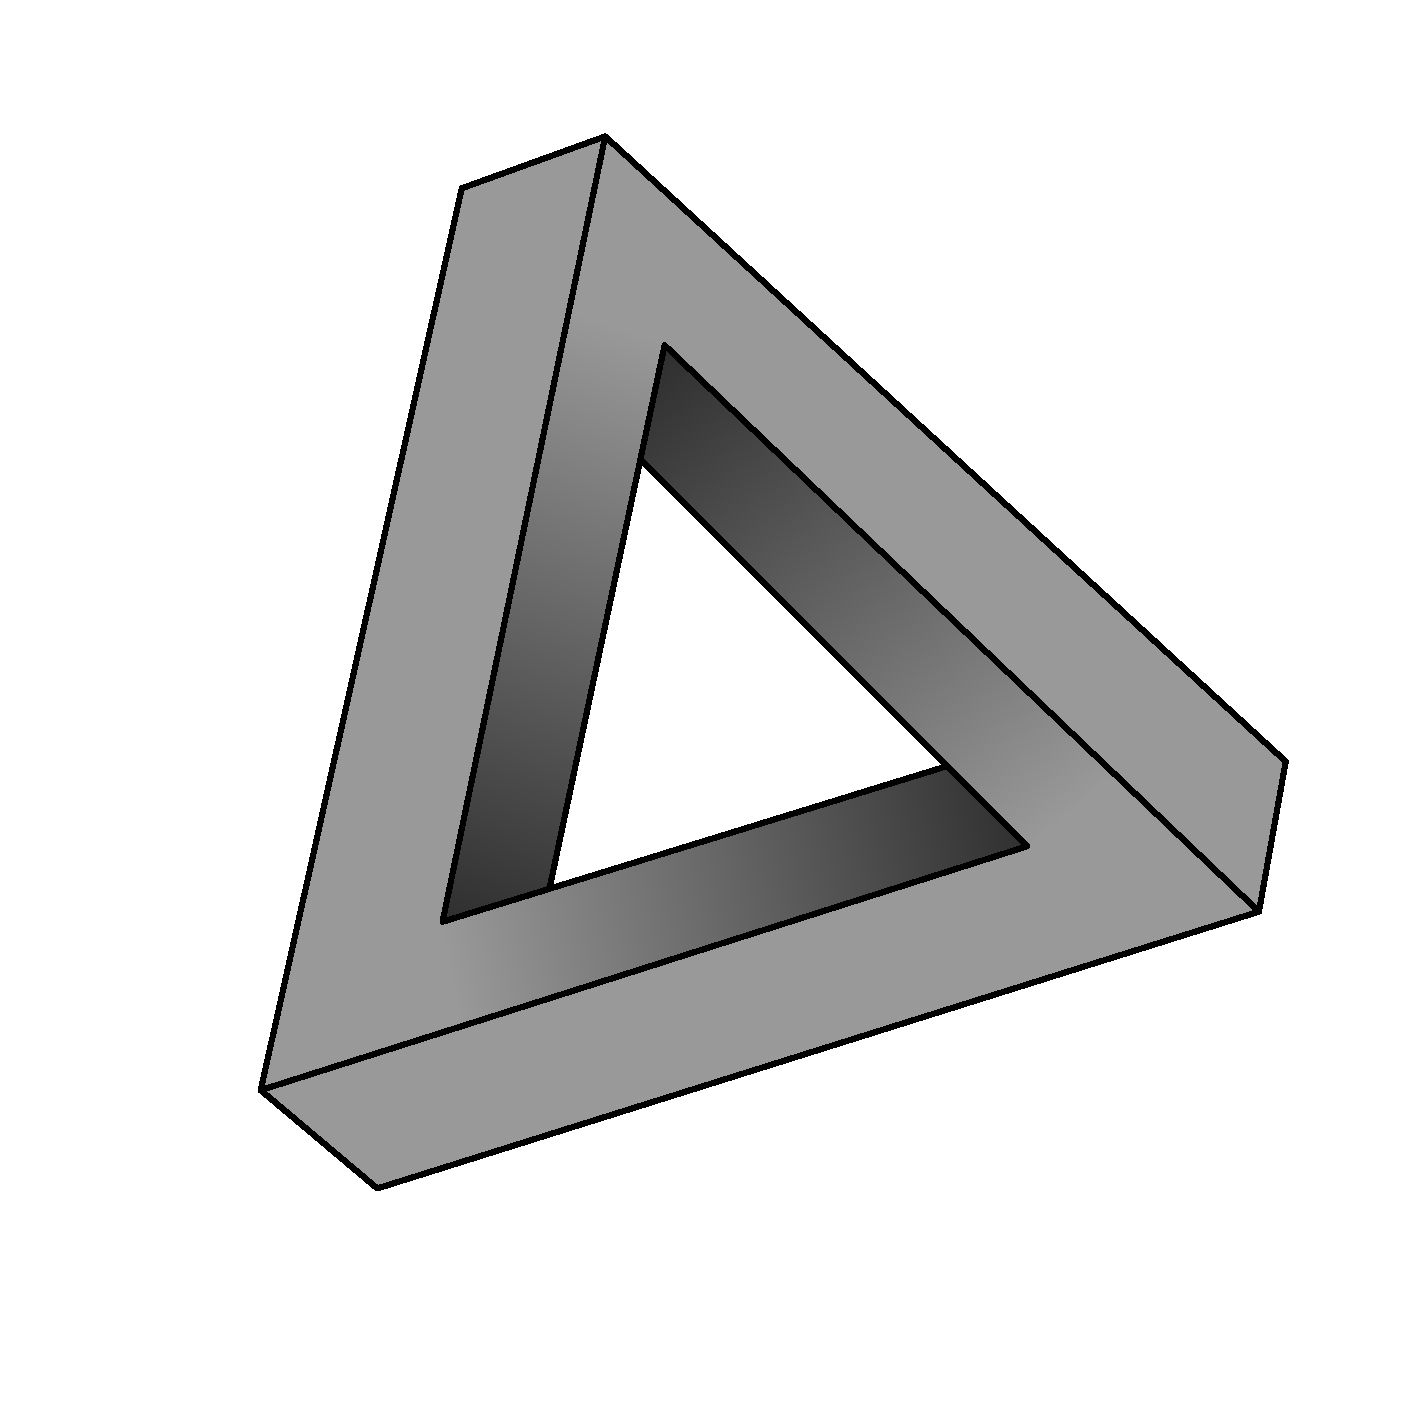
\includegraphics[scale=.25]{../Images/tribar_ombre.pdf}
\end{center}
\nota{Bonjour, je m'appelle Basile Pillet et je suis doctorant à l'institut de mathématiques de Rennes. Je vais vous parler d'un outil assez sophistiqué d'algèbre et de géométrie qu'on appelle \textit{Cohomologie} et je vais vous le présenter sur l'exemple du \textit{triangle de Penrose}.}
\nota{Le \textit{triangle de Penrose}, c'est l'objet impossible dessiné ici. Il a été créé par le physicien et mathématicien Sir Roger Penrose dans les années 50. Il a alors été présenté comme étant "\textit{L'impossibilité dans sa forme la plus pure}".}
\nota{On va se servir de la cohomologie pour identifier ce qui empêche un tel objet d'exister.}
\end{frame}


\newgeometry{margin=0pt}

\begin{frame}% POSSIBLE LOCALEMENT
\begin{center}
\nota{On part de notre objet impossible}
\includegraphics<1|handout:0>[scale=.4]{../Images/tribar.pdf}
\nota{Si on ne regarde que le coin en haut à gauche ...}
\includegraphics<2>[scale=.4]{../Images/UpperCorner.pdf}
\nota{... on remarque qu'il n'a plus rien d'impossible !}
\includegraphics<3|handout:0>[scale=.4]{../Images/UpperCorner2.pdf}
\nota{On peut le réaliser en vrai avec deux bouts de bois et un peu de colle}
\includegraphics<4|handout:0>[scale=.4]{../Images/UpperCorner3.pdf}
\end{center}
\end{frame}


\begin{frame}% Recouvrement
\begin{center}
\nota{Revenons à notre \textit{triangle de Penrose} ou plutôt son dessin}
\includegraphics<1|handout:0>[scale=.4]{../Images/tribar.pdf}
\nota{On peut découper ce dessin en trois parties autour de chaque coin.}
\includegraphics<2|handout:0>[scale=.4]{../Images/Covering.pdf}
\nota{...parties qui s'intersectent}
\includegraphics<3>[scale=.4]{../Images/Covering2.pdf}
\end{center}
\end{frame}


\begin{frame}% Split
\begin{center}
\nota{Éclatons donc notre dessin. On a trois dessins qui chacun représente des objets RÉALISABLES}
\includegraphics<1>[scale=.4]{../Images/Covering_split.pdf}
\nota{Ces trois dessins doivent être recollés suivant les zones rouges pour obtenir le dessin d'origine.}
\nota{Notre figure impossible est LOCALEMENT possible. Mais si les trois dessins peuvent se recoller pour donner le dessin du \textit{triangle de Penrose}, les trois objets physiques eux ne peuvent pas ! C'est ce qu'on va voir.}
\end{center}
\end{frame}


\begin{frame}% Notations
\begin{center}
\nota{Appelons $U_1$, $U_2$ et $U_3$ les trois parties qui recouvrent le dessin. Prenons un point $A$ sur le dessin qui soit à la fois dans $U_1$ et $U_2$}
\includegraphics<1|handout:0>[scale=.4]{../Images/A.pdf}
\nota{Après découpage, le point $A$ se dédouble : une copie $A_{1}$ dans $U_1$ et une copie $A_{2}$ dans $U_2$}
\includegraphics<2>[scale=.4]{../Images/Ai.pdf}
\end{center}
\end{frame}


\begin{frame}% Distance observateur
\begin{center}
\nota{
Si maintenant on construit un coin numéro $1$, il aura une certain taille. Et pour qu'il apparaisse tel que sur le dessin, il faut le mettre à une certaine distance de l'observateur. Si on l'avait construit plus petit, il aurait fallu le mettre plus près.
}
\includegraphics<1>[scale=.5]{../Images/DistanceObservateur2.pdf}
\nota{
Mais le coin numéro $2$ n'est pas forcément à la même distance de l'observateur. Imaginez que l'on construise l'objet $1$ immense mais très loin et l'objet $2$ petit mais très près.
}
\includegraphics<2|handout:0>[scale=.4]{../Images/1Loin2Pres_.pdf}
\end{center}
\end{frame}


\begin{frame}% Dij
\nota{
Pour garder cette information en mémoire, on va noter $d_{12}$ le rapport des distances entre ces deux points.
}
\begin{equation*}
d_{12} = \alt<2>{\dfrac{OA_1}{OA_2}}{\dfrac{\text{ distance du point représenté par }A_{1}\text{ à l'observateur}}{\text{ distance du point représenté par }A_{2}\text{ à l'observateur}}}
\end{equation*}
\end{frame}

\begin{frame}% 6 points
\begin{center}
\nota{
On recommence avec un point $B$ sur l'intersection de $U_1$ et $U_3$ et un point $C$ sur l'intersection de $U_2$ et $U_3$
}
\includegraphics<1>[scale=.4]{../Images/6points.pdf}
\end{center}
\end{frame}

\begin{frame}% Dij
\begin{center}
\begin{equation*}
d_{12} = \dfrac{OA_1}{OA_2}
\end{equation*}
\nota{On définit de même entre l'objet $1$ et l'objet $3$ le rapport $d_{31}$}\pause
\begin{equation*}
d_{31} = \dfrac{OB_{3}}{OB_{1}}
\end{equation*}
\nota{et le rapport $d_{23}$}\pause
\begin{equation*}
d_{23} = \dfrac{OC_{2}}{OC_{3}}
\end{equation*}
\end{center}
\end{frame}


\begin{frame}% Recollement
\begin{center}
\frametitle{\hfill Recollement}
\nota{À quelle(s) condition(s) les trois objets construits se recollent-t-ils ?}
Pour se recoller \\
\pause
\bigskip
il faut \nota{Il faut}
\medskip
\begin{itemize}[<+->]
\item que $A_1$ et $A_2$ se superposent\nota{que $A_1$ et $A_2$ se superposent ... donc qu'ils soient à la même distance de l'observateur}%
\uncover<5->{ : \quad  $d_{12} = 1$} \nota{... donc que le rapport $d_{12}$ vaille $1$.}
\item que $B_1$ et $B_3$ se superposent\uncover<6->{ :  \quad  $d_{31} = 1$}
\item que $C_2$ et $C_3$ se superposent\uncover<7->{ :  \quad  $d_{23} = 1$}
\end{itemize}
\end{center}
\end{frame}


\begin{frame}% inception
\begin{center}
\nota{
Ces conditions sont nécessaire pour que l'objet existe réellement. Sinon on pourrait avoir des problèmes comme dans le film Inception. 
}
\vspace*{-1.9em}
\includegraphics<1>[width=1.1 \paperwidth]{../Images/Inception.jpg}
\hspace*{-8em}\includegraphics<2|handout:0>[width=1.8 \paperwidth]{../Images/Inception2.jpg}
\end{center}
\end{frame}

\section{Homothétie}

\begin{frame}% Homothétie
\begin{center}
\nota{Que voyons-nous ?}
\includegraphics<1|handout:0>[scale=.4]{../Images/ABC.pdf}
\includegraphics<2>[scale=.4]{../Images/d12d23d31.pdf}
\only<3>{Les $d_{ij}$ forment un \textbf{cocycle}.}
\nota{C'est l'information importante sur cette construction.}
\end{center}
\end{frame}

\begin{frame}% Homothétie 2
\begin{center}
\only<1>{Que ce passe-t-il si on multiplie toutes les dimensions de l'objet $1$ par $\lambda_1 \in \R^{+*}$ ainsi que sa distance à l'observateur ?}
\nota{Rien ne change}
\includegraphics<2>[scale=.4]{../Images/ABC.pdf}
\end{center}
\end{frame}


\begin{frame}% Homothétie 2
\begin{center}
\nota{Cependant}
\begin{align*}
d_{12} & \mapsto \uncover<2->{\lambda_1 d_{12}} \\[2em]
d_{31} & \mapsto \uncover<3->{\dfrac{d_{31}}{\lambda_1}} \\[2em]
d_{23} & \mapsto \uncover<4->{d_{23}}
\end{align*}
\end{center}
\end{frame}



\begin{frame}% Homothétie 2
\nota{}
\begin{center}
Il existe une manière de redimensionner les trois objets telle que 
\[
d_{12} = d_{23}= d_{31}  = 1
\] \pause
( c'est-à-dire de recoller les trois coins en un vrai \textit{triangle de Penrose} )\\
\bigskip\pause
si et seulement si\\
\bigskip\pause
\begin{equation*}
d_{12} = \dfrac{\lambda_1}{\lambda_2} \quad , \qquad d_{31} = \dfrac{\lambda_3}{\lambda_1} \quad  , \qquad d_{23} = \dfrac{\lambda_2}{\lambda_3}
\end{equation*}
\pause
\bigskip
on dit alors que les $d_{ij}$ forment un \textbf{cobord}.
\end{center}
\end{frame}


\begin{frame}
  \frametitle{\hfill Le \textit{triangle de Penrose} existe \\
    \hfill ssi\\
    \hfill les $d_{ij}$ forment un cobord}
  \nota{Donc le \textit{triangle de Penrose} existe si et seulement si les $d_{ij}$ forment un cobord.}
  \pause
\begin{center}
Si c'est le cas alors
\[
d_{12} \times d_{23} \times d_{31}= \pause
\dfrac{\lambda_1}{\lambda_2} \times \dfrac{\lambda_2}{\lambda_3} \times  \dfrac{\lambda_3}{\lambda_1}= \pause
1
\]
\end{center}
\end{frame}

\iffalse
\begin{frame}
\begin{center}
\nota{Si l'on regarde l'ensemble des triplet $d_{12},d_{31}, d_{23}$ mais qu'on force ceux qui s'écrivent comme des quotients de $\lambda_i$ à s'annuler on a construit un objet de ce qu'on appelle \textbf{espace de cohomologie}}
\[
H^1(U, \R^{+*}) = \dfrac{\left\{\text{triplets }(d_{12},d_{31}, d_{23})\right\}}{\left\{\text{triplets }(d_{12},d_{31}, d_{23}) \text{ tels que }d_{ij} = \lambda_i/\lambda_j\right\}}
\]
\end{center}
\end{frame}
\fi

\section{Contradiction}


\begin{frame}% Contradiction
\nota{On va montrer que c'est absurde}
\begin{center}
\includegraphics<1>[scale=.4]{../Images/ABC.pdf}
\includegraphics<2|handout:0>[scale=.4]{../Images/A1<B1.pdf}
\note[item]{On voit que le point $A_1$ est plus proche que le point $B_1$}
\only<2,3,5,7>{
\[
OA_1 < OB_1
\]}
\includegraphics<4|handout:0>[scale=.4]{../Images/B3<C3.pdf}
\note[item]{Le point $B_3$ est plus proche que le point $C_3$}
\only<5,7>{
\[
OB_3 < OC_3
\]}
\includegraphics<6|handout:0>[scale=.4]{../Images/A2>C2.pdf}
\note[item]{Le point $C_2$ est plus proche que le point $A_2$}
\only<7>{
\[
OC_2 < OA_2
\]}
\end{center}
\end{frame}

\begin{frame}
\nota{En regroupant tout ça}
\begin{center}
\begin{align*}
1 &= d_{12} \times d_{23} \times d_{31}\\
\uncover<2->{&= \dfrac{OA_1}{OA_2} \times \dfrac{OC_2}{OC_3} \times \dfrac{OB_3}{OB_1}\\ }
\only<3>{&= \dfrac{OA_1}{OB_1} \times \dfrac{OC_2}{OA_2} \times \dfrac{OB_3}{OC_3}\\ }
\uncover<4->{&= \underset{<1}{\underbrace{\dfrac{OA_1}{OB_1}}} \times \underset{<1}{\underbrace{\dfrac{OC_2}{OA_2}}} \times \underset{<1}{\underbrace{\dfrac{OB_3}{OC_3}}}\\ }
\uncover<5->{&< 1\\  }
\end{align*}

\uncover<6->{Le \textit{triangle de Penrose} n'existe pas.}
\end{center}
\end{frame}

\iffalse
\begin{frame}
\nota{En regroupant tout ça}
\begin{center}
\begin{align*}
d_{13} &= d_{12} \times d_{23}\\
\uncover<2->{&= \dfrac{\text{distance}(A_1)}{\text{distance}(A_2)} \times \dfrac{\text{distance}(C_2)}{\text{distance}(C_3)}\\ }
\uncover<3->{&< \dfrac{\text{distance}(A_1)}{\text{distance}(C_2)} \times \dfrac{\text{distance}(C_2)}{\text{distance}(C_3)}\\ }
\uncover<4->{&< \dfrac{\text{distance}(A_1)}{\text{distance}(C_3)}\\  }
\uncover<5->{&< \dfrac{\text{distance}(B_1)}{\text{distance}(C_3)}\\  }
\uncover<6->{&< \dfrac{\text{distance}(B_1)}{\text{distance}(B_3)}\\  }
\uncover<7->{&< d_{13} }\\
\end{align*}

\uncover<8->{Le \textit{triangle de Penrose} n'existe pas.}
\end{center}
\end{frame}

\begin{frame}
\nota{En regroupant tout ça}
\begin{center}
\begin{align*}
  d_{13} \times \text{distance}(C_3) \uncover<1->{&= d_{12} \times d_{23} \times \text{distance}(C_3)\\  }
  \note[item]{Condition de cocycle}
														  \onslide*<2>{&= d_{12} \times \dfrac{\text{distance}(C_2)}{\text{distance}(C_3)}\times \text{distance}(C_3)\\ }
														  \uncover<3->{&=  d_{12} \times\text{distance}(C_2)\\ }
													      \uncover<4->{&<  d_{12} \times\text{distance}(A_2)\\  }
  \note[item]{Car $C_2$ est plus proche que $A_2$}
                                                              \onslide*<5>{&<  \dfrac{\text{distance}(A_1)}{\text{distance}(A_2)}\times\text{distance}(A_2)\\ }
  \note[item]{En simplifiant}
                                                              \uncover<6->{&< \text{distance}(A_1)\\ }
  \note[item]{Car $A_1$ est plus proche que $B_1$}
                                                              \uncover<7->{&< \text{distance}(B_1)\\  }
                                                              \onslide*<8>{&= \dfrac{\text{distance}(B_1)}{\text{distance}(B_3)} \times \text{distance}(B_3)\\  }
                                                              \uncover<9->{&= d_{13} \times \text{distance}(B_3)\\ }
                                                              \uncover<10->{&< d_{13} \times \text{distance}(C_3) \\ }
  \note[item]{Car $B_3$ est plus proche que $C_3$.}
\end{align*}

\uncover<11->{Le \textit{triangle de Penrose} n'existe pas.}
\end{center}
\end{frame}
\fi

\begin{frame}
\begin{center}
\nota{L'intérêt n'est pas de montrer que le \textit{triangle de Penrose} est impossible ! L'intérêt c'est qu'en mathématique (en algèbre et en géométrie), quand quelque chose ne marche pas, eh bien la vie ne s'arrête pas. Il y a \textbf{des choses}, de nouveaux objets, qui empêchent que ça marche et l'étude de ces \textbf{obstructions} se révèle bien souvent très riche}\vspace*{-2.5em}
\hspace*{-6em}\includegraphics<1>[scale=.87]{../Images/lego-triangle.jpg}
\end{center}
\end{frame}


\appendix

\begin{frame}
\begin{center}
\begin{itemize}
\item \textsc{Roger Penrose}, \textit{On the Cohomology of Impossible Figures.}\\ \quad Leonardo 25, no. 3/4 Visual Mathematics: Special Double Issue (\textbf{1992}), pp. 245-247\\
\end{itemize}
\end{center}

\end{frame}

\end{document}
